%
% File twocolumn.tex
%
%%
%% Based on the style files for *SEM-2014, which were, in turn,
%% Based on the style files for COLING-2014, which were, in turn,
%% Based on the style files for ACL-2014, which were, in turn,
%% Based on the style files for ACL-2013, which were, in turn,
%% Based on the style files for ACL-2012, which were, in turn,
%% based on the style files for ACL-2011, which were, in turn,
%% based on the style files for ACL-2010, which were, in turn,
%% based on the style files for ACL-IJCNLP-2009, which were, in turn,
%% based on the style files for EACL-2009 and IJCNLP-2008...

%% Based on the style files for EACL 2006 by
%%e.agirre@ehu.es or Sergi.Balari@uab.es
%% and that of ACL 08 by Joakim Nivre and Noah Smith

\documentclass[11pt]{article}
\usepackage{semeval2014}
\usepackage{times}
\usepackage{url}
\usepackage{latexsym}
\usepackage{color}
\usepackage[usenames,dvipsnames,svgnames,table]{xcolor}
\usepackage{amsmath}
\usepackage{bm}
\usepackage{amssymb}
\usepackage{graphicx}
\usepackage{enumitem}
\usepackage{multirow}
\usepackage{tabularx}
\usepackage{subcaption}

\setitemize{noitemsep,topsep=10pt,parsep=0pt,partopsep=0pt}
\setenumerate{noitemsep,topsep=10pt,parsep=0pt,partopsep=0pt}

%\setlength\titlebox{5cm}

% You can expand the titlebox if you need extra space
% to show all the authors. Please do not make the titlebox
% smaller than 5cm (the original size); we will check this
% in the camera-ready version and ask you to change it back.

\newcommand{\wsname}{SemEval-2014}
\newcommand{\submissionpage}{\url{http://alt.qcri.org/semeval2014/index.php?id=cfp}}
\newcommand{\filename}{semeval2014}
\newcommand{\contact}{pnakov qf.org.qa}


\definecolor{myblue}{rgb}{0,0.1,0.6}
\definecolor{mygreen}{rgb}{0,0.3,0.1}
\usepackage[colorlinks=true,linkcolor=black,citecolor=mygreen,urlcolor=myblue]{hyperref}
\newcommand{\transpose}{^\mathsf{T}}

\newcommand{\bocomment}[1]{\textcolor{Bittersweet}{[#1 -BTO]}}
\newcommand{\sam}[1]{\textcolor{blue}{[#1 -SMT]}}
\newcommand{\jdcomment}[1]{\textcolor{NavyBlue}{[#1 -JDD]}}

% turn off for submission, but on for a more tech report-y version.
\newcommand{\codenote}[1]{\textcolor{PineGreen}{[#1]}}
\newcommand{\logitedge}{\textsc{LogitEdge}}
\newcommand{\noedge}{\textsc{NoEdge}}

% saves only a little bit of space. might need tweaking to save more.
\newenvironment{itemizesquish}{\begin{list}{\labelitemi}{\setlength{\itemsep}{-0.1em}\setlength{\labelwidth}{1em}\setlength{\leftmargin}{\labelwidth}\addtolength{\leftmargin}{\labelsep}}}{\end{list}}


\title{CMU-Ark: Broad-Coverage Semantic Dependency Parsing with Rich
Edge-Factored Features \sam{better title, please}}

\author{First Author \\
  Affiliation / Address line 1 \\
  Affiliation / Address line 2 \\
  Affiliation / Address line 3 \\
  {\tt email@domain} \\\And
  Second Author \\
  Affiliation / Address line 1 \\
  Affiliation / Address line 2 \\
  Affiliation / Address line 3 \\
  {\tt email@domain} \\}

\date{}

\begin{document}
\maketitle

\begin{abstract}
We present an edge-factored statistical model for parsing to the three semantic
dependency formalisms in SemEval 2014 Shared Task 8: Broad-Coverage Semantic
Dependency Parsing.

\end{abstract}



\section{Introduction}

The task of broad coverage semantic dependency parsing aims to provide a
shallow semantic analysis of text not limited to a specific domain.
As distinct from deeper semantic analysis (e.g., parsing to a full
lambda-calculus logical form), shallow semantic parsing captures relationships
between pairs of words or concepts in a sentence, and has wide application for
information extraction, knowledge base population, and question answering (among others).
SemEval 2014 Shared Task 8: Broad-Coverage Semantic Dependency
Parsing \cite{oepens_broad_2014} includes three different semantic
formalisms (\S\ref{s:formalisms}), which encourages finding features and methods
that are broadly applicable to semantic parsing, and discourages optimization
toward a single semantic representation.
By diversifying the representations, we better tackle the broader task of
semantic analysis itself.

We present here two systems that produce semantic dependency parses by extracting
features for each potential dependency arc and learning a statistical model to
discriminate between good arcs and bad;
the first treats each labeled edge decision as an independent multiclass
logistic regression (\S\ref{s:logitedge}), while the second predicts all edges
as part of a graph-based structured SVM (\S~\ref{s:graphparser}). 
Common to both models are a rich set of edge features, described in
\S\ref{s:edgefeatures}.
While the features included in the final prediction were all found to have a
positive impact on the final development accuracy, we also describe a range of
other features (\S\ref{s:badfeatures}) found to have no discernable impact (or
even negative impact) in our development.

Our system placed second in the open track of the broad-coverage semantic
parsing task (in which output from syntax parsers and other outside resources can be used).
We present our results, and compare to the first place system, PRIB-IT
\cite{martins_prib_2014}, in \S\ref{s:evaluation}.



\section{Formalisms} \label{s:formalisms}

The organizers of Shared Task 8 have provided a corpus of English language
newswire annotated with three different semantic dependency formalisms.
%Here we briefly describe the three formalisms, and refer the reader to \sam{the
%shared task paper, cite} for a more complete summary.
\emph{DM} is automatically derived from LinGO English Resource Grammar (ERG)
annotations in DeepBank \cite{flickinger_deepbank_2012}.
\emph{PAS} is automatically derived from the Enju HPSG treebank using the
conversion rules of \newcite{miyao_corpus_oriented_2004}.
And \emph{PCEDT} is automatically derived from the tectogrammatic layer of the
Prague Czech--English Dependency Treebank \cite{hajic_building_1998}.
See Figure~\ref{fig:formalisms} for an example sentence.
\begin{figure*}
	\centering
	\begin{subfigure}{0.7\textwidth}
		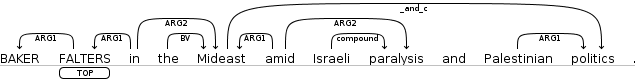
\includegraphics[width=\textwidth]{fig/example_dm}
		\caption{DM}
		\label{fig:dm}
	\end{subfigure}
	\begin{subfigure}{0.7\textwidth}
		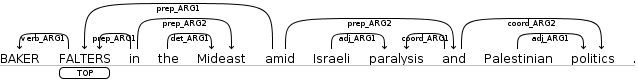
\includegraphics[width=\textwidth]{fig/example_pas}
		\caption{PAS}
		\label{fig:pas}
	\end{subfigure}
	\begin{subfigure}{0.7\textwidth}
		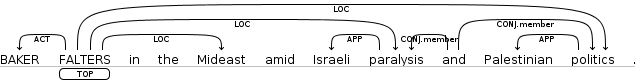
\includegraphics[width=\textwidth]{fig/example_pcedt}
		\caption{PCEDT}
		\label{fig:pcedt}
	\end{subfigure}
	\caption{Example annotations for the three formalisms.}
	\label{fig:formalisms}
\end{figure*}

All three formalisms come from very different linguistic theories, but all
three are represented as labeled directed graphs, with words as vertices, and
all three have ``top'' annotations\footnote{
``Top'' annotations roughly correspond to the semantic focus of a
sentence, but there is no constraint that the ``top'' must be a root of the
semantic dependency graph.}.
This allows us to use the same machinery (\S\ref{s:models}) to simultaneously
train and test statistical models for the three formalisms.
\sam{Stats about \% multiple roots, \% multiple tops, \% tree, \% acyclic}



\section{Models} \label{s:models}

We treat the problem as a three-stage pipeline.
The first stage prunes words by predicting whether a word is a \emph{singleton}
or not--whether it has any incoming or outgoing edges at all (\S\ref{s:singleton_model}).
If a word is predicted to be a singleton, then it no longer needs to be
considered in later stages.
The second stage jointly predicts whether an edge is
present, and if so, what its label is (\S\ref{s:edge_model}).
The third stage predicts whether a word is a \emph{top} or not
(\S\ref{s:top_model}).
Formalisms sometimes annotate more than one ``top'' per sentence, but we
found that we achieve the best performance on all formalisms by predicting only
the one best-scoring ``top'' under the model.
\bocomment{I thought that only LogitEdge has the separate third stage of ``top'' prediction. Maybe I'm wrong? delete this comment if so}
\bocomment{Also, singleton pruning does not matter for LogitEdge.  It doesn't affect accuracy, I'm pretty sure.  But it is essential for the graph model.}


\subsection{Singleton Classification} \label{s:singleton_model}

We call a node in a graph without any parents or children a \emph{singleton}.
For singleton prediction, we train a simple token-level logistic regression
classifier.
We train a model for each of the three formalisms, as each of the three
formalisms follow different conventions determining whether a token would be
included in the final graph for a sentence.
The PAS formalism, for example, includes almost all tokens that are not
punctuation or a determiner, and our singleton model achieves over 99\%
accuracy.
\jdcomment{I need to find the accuracy for the other two formalisms. Will
include this in our Results section.}

For each token $t$, the model considers the following features:
\begin{itemize}
\item the token $t$ itself
\item the lemma of $t$
\item the part of speech tag of $t$
\end{itemize}



\subsection{Edge Prediction} \label{s:edge_model}

In the second stage of the pipeline, we predict the set of labeled directed
edges in the graph.
We use the same set of edge-factored features (\S\ref{s:features}) in two
different models.
For the DM and PCEDT formalisms, we use an edge-independent multiclass logistic
regression model (\logitedge, \S\ref{s:logitedge}).
For the PAS formalism, we use a structured SVM 
\cite{taskar_max_2003,tsochantaridis_support_2004} that enforces a
\emph{determinism} constraint -- a word may not have two outgoing edges with the
same label (\S\ref{s:graphparser}).
\sam{explain why we use different models for different formalisms}
\bocomment{shouldn't we just say, we tried both for all and are reporting the configurations that performed best on devset?}
\sam{yes, that sounds good. waiting on graph vs. non-graph results from jflan}

Both models consider only token index pairs $(i, j)$ where %that are within 10
% tokens of each other (i.e.~
$|i-j| \leq 10$, $i \ne j$, and both $i$ and
$j$ have been predicted to be non-singletons by the first stage.
In other words, edges with more than 9 tokens between its two endpoints are not
considered.
Although this prunes some gold edges, among the formalisms,
95\%-97\% of all gold edges are between tokens of distance 10 or less.
We found that pruning long edges increased accuracy overall, in addition to
speeding up training and prediction.
Both directions $i \rightarrow j$ and $j \rightarrow
i$ are considered between every pair.


\subsubsection{\logitedge\ parser} 
\label{s:logitedge}


\codenote{LRParser.java}

%\noindent
The \logitedge\ model treats every ordered pair of token indices $(i, j)$ as a
multiclass logistic regression with $K+1$ possible outputs:
the formalism's original $K$ edge labels plus the additional label \noedge,
which indicates that no edge exists from $i$ to $j$.
Let $L$ be the set of possible edge labels.

In our implementation, we separate features into two classes:
those which can be extracted for any one word, $\bm{f}^{(\text{node})}(i)$;
and those which look at both the parent and the child,
$\bm{f}^{(\text{edge})}(i, j)$.
These features are described in \S\ref{s:features}.
The final binary feature vector is made by conjoining the output label with
each:
\bocomment{we dont always use binary features...}
\begin{align*} 
\bm{f}(i, j, \ell) =
\{ \ell \} \otimes (& 
	\{ \text{``bias''} \} \\
	& \cup \bm{f}^{(\text{edge})}(i, j) \\
	& \cup \{ \text{``parent''} \} \otimes \bm{f}^{(\text{node})}(i) \\
	& \cup \{ \text{``child''} \} \otimes \bm{f}^{(\text{node})}(j)
)\\
\end{align*}
\noindent
where  $\otimes$ represents the Cartesian product.
%Feature extractors are defined to extract
%features both for individual tokens ($f^{(\text{node})}(i)$), and also for
% pairs of tokens ($f^{(\text{edge})}(i,j)$), which are conjoined against all possible output
%labels.
For candidate parent index $i$ and child index $j$, the model defines a
distribution over $y_{i,j} \in L$, parametrized by the weight vector $\bm\phi$,

\begin{equation}
  Pr(y_{i,j}=\ell; \bm\phi)  = \frac{
  	e^{\bm\phi^\top \bm{f}(i, j, \ell)}
  } {
  	\sum_{\ell^\prime \in L} {
  		e^{\bm\phi^\top \bm{f}(i, j, \ell^\prime)}
  	}
  }
\end{equation}

\noindent
%In this notation, an $f$ function outputs a real-valued vector, defined as the
% concatenation of features from all the feature classes (\S\ref{s:features}).
$\bm\phi$ is learned by minimizing total negative log-likelihood of the above
(with weighting; see below), plus $\ell_2$ regularization.
Adagrad \cite{duchi_adaptive_2011} is used for optimization.
It seemed to optimize faster than L-BFGS \cite{byrd_limited_1995}, at least for earlier
iterations, though we did no systematic comparison. Stochastic gradient steps are applied one at a time from individual examples, and a gradient step for the regularizer is applied once per epoch.

In the FFF formalism, the training set (\S\ref{s:evaluation})
contains NNN candidate edges (pairs of tokens with length between 1 and 10 inclusive),
and NNN actual (non-null) edges.  $F_1$ performance was improved by
downweighting $\noedge$ examples through a weighted log-likelihood objective,
$\sum_{i,j} \sum_\ell w_\ell \log P(y_{i,j}=\ell; \bm\phi)$, with $w_{\noedge}=0.3$
and $1$ otherwise.
(The weight was chosen by gridsearch on a development set; 
PAS used a weight of $0.4$ while the others were $0.3$, though the differences at this granularity were small.)

% Besides the edge logistic regression system, there were both pre- and post-processing steps.

% \textbf{Preprocessing:}
% \bocomment{TODO need to check how much preproc was used for this.  Was singleton pruning turned on?  It looks like we commented out the prune features in LRParser.java.  But singleton pruning might have been turned on.}

% \textbf{Decoding and postprocessing:}
\textbf{Decoding:}
\codenote{decodeEdgeProbsToGraph(), MyGraph.java}

To predict a graph structure at test-time for a new sentence,
the most likely edge label is predicted for every candidate $(i, j)$ pair of
tokens that has not been pruned by an earlier stage.
We enforce only one graph constraint, which is that there cannot be
an edge in both directions between any pair of words.
If an edge is predicted for both directions for a single $(i, j)$
pair, only the edge with the higher score is chosen.
There are no such bidirectional edges in the training data, and enforcing this
restriction slightly improved accuracy on the development set ($~0.2\%$ absolute F on PAS; other formalisms unchanged).\codenote{\url{https://github.com/Noahs-ARK/semeval-2014/pull/21}}


\subsubsection{Graph-based Structured SVM Parser} \label{s:graphparser}

To predict edges for the PAS formalism, we use a structured SVM model
\sam{cite}.
The model uses the same set of features as \logitedge, but optimizes a
max-margin objective during training, and enforces an additional constraint: no
node may have more than one outgoing edge with the same label.

\sam{TK from jflan}

\sam{
explain how this differs from 
\cite{flanigan-etal:ACL2014}
}

\bocomment{Does this use the topness prediction system?}



\subsubsection{Edge Features}
\label{s:edgefeatures}

\label{s:features}
These features were computed over an edge $e$ with parent token $s$ at index
$i$ and child token $t$ at index $j$. 
For each feature listed, we have an indicator feature for each value it takes
on.

\begin{itemize}
	\item Basic
	\begin{itemize}
		\item The tokens $s$ and $t$ themselves.
		\item Lemmas of $s$ and $t$.
		\item Part of speech tags of $s$ and $t$.
		\item 1 if $i \le j$, 0 otherwise.
	\end{itemize}
	\item LinearOrder
		\begin{itemize}
		\item $i - j$.
	\end{itemize}
	\item CoarseDependency
		\begin{itemize}
		\item 1 if $s$ is the parent of $t$ in the syntactic dependency parse, 0
		otherwise.
		\item Distance between $s$ and $t$ in syntactic dependency parse.
	\end{itemize}
	\item LinearContext
		\begin{itemize}
		\item Concatenated POS tags of tokens at $i-1$, $i$, $i+1$, $j-1$, $j$,
		and $j+1$.
		\item Concatenated POS tags of tokens at $i-1, i, j-1$, and $j$.
		\item Concatenated POS tags of tokens at $i, i+1, j$, and $j+1$.
	\end{itemize}
	\item DependencyPath
		\begin{itemize}
		\item The concatenation of all tokens and arc labels on the labeled path in
		the syntactic dependency tree from $s$ to $t$.
	\end{itemize}
	\item UnlabeledDep
		\begin{itemize}
		\item The unlabeled path through the syntactic dependency tree from $s$ to $t$. 
		\item The unlabeled path through the syntactic dependency tree from $s$ to $t$,
		annotated with whether the each step through the tree was to the right or left in the sentence.
	\end{itemize}
	\item SubcatSequence
		\begin{itemize}
		\item For each direct child $c$ of $s$ in the syntactic dependency tree, the
		concatenation of the POS tag of $c$ with the label of the arc to the child.
		If $c$ is $t$, append a ``+''.
		\item For each child $c$ of $s$ in the syntactic dependency tree, the
		concatenation of the POS tag of $s$ with the POS tag of $c$ and the label of the
		arc from $s$ to $c$.
		If $c$ is $t$, append a ``+''.
	\end{itemize}
\end{itemize}

\subsubsection{Feature Hashing}

\bocomment{ALTERNATE VERSION TO SAVE SPACE:
  The biggest memory usage was in the hash table implementing the map of feature names to integer indexes, used during feature extraction.  In order to facilitate more convenient experimentation, we implemented multitask feature hashing \cite{weinberger_feature_2009}, which randomly assigns features' numeric indexes with a hash function, under the theory that errors due to collisions tend to cancel each other out.  We indeed found no drop in accuracy when using the technique.}

%% 7-10 million features (percepts) before label conjunction:
% cab:~dbamman/semeval/mar3 % wc -l *.model
%    7518732 mar3_recsplit.dm.model
%    7038841 mar3_recsplit.pas.model
%    9939549 mar3_recsplit.pcedt.model
%   24497122 total

\codenote{
\url{https://github.com/Noahs-ARK/semeval-2014/pull/20}
Code:
  See use of flag LRParser.useHashing, esp LRParser::perceptNum() 
  and Model::coefIdx(): hashed values before and after label conjunction.
}

\noindent
For \logitedge, the biggest memory usage was from
the hash table that implemented
a map of feature names to integer indexes, used during feature extraction.
Tens of millions of features (before conjunction) resulted in several gigabytes of memory use.  To facilitate more convenient experimentation,
we eliminated this by using
multitask feature hashing
\cite{weinberger_feature_2009},
which randomly assigns features' numeric indexes with a hash function.\footnote{We also tried replacing the hash table with a Patricia Tree, trying several open-source implementations; but they had worse memory usage than a GNU Trove hash table. 
  \codenote{\url{https://github.com/brendano/myutil/blob/0a5697a7f066c265a75ce1b7bd527feafa683c8a/src/vocabalts/vocabalts_results.txt}}}
Let $F$ be the space of all feature names (before conjunction with the output label).
In the usual approach, a hash table is maintained containing a
one-one onto map from features to integer indexes $g: F \rightarrow \{1,\ldots,|F|\}$,
and each output label has an array of model parameters $\bm\phi^\ell \in \mathbb{R}^{|F|}$,
which $g(f)$ indexes into.
In the hashing approach, a hash function $h_{\ell}$
maps feature name to one of $B$ bucket values,
$h_{\ell} : F \rightarrow \{1, \ldots, B\}$.
(A different hash function is used for each output label.)
The model parameters are stored in an array $h_\ell(\bm\phi^\ell) \in \mathbb{R}^{B}$,
for which an entry is defined as
\[
  h_\ell(\bm\phi^\ell)_{b} = 
  \sum_{\substack{\text{feat} \in F 
    \\\text{ s.t. } h_\ell(\text{feat})=b}}
  {\phi^\ell_{\text{feat}}}
\]
This is easy to implement:
array lookups and gradient steps are simply implemented with $h$ instead of $g$, and feature vectors are also stored in a hashed space.
\cite{weinberger_feature_2009} show that, even with some collisions,
dot products are approximately preserved with high probability;
and indeed, we observed no drop in accuracy compared to using an explicit feature map.
We used a value of $B$ as large as was convenient for memory usage (due only to $h(\phi)$), $B=10^{8}$.
This was actually higher than $|F|\approx 10^7$, though there were still plenty of collisions: about 9.5\% of features are hashed to a value shared by at least one other feature.

%% simulation:
% num buckets count 0: 90484843
% num buckets count 1: 9046266
% num collisions: num features that are in a non-singleton bucket: 953734
%%  average over simulations for last value: 9.518e+05 


\subsection{Top Prediction} \label{s:top_model}

We trained a separate token-level binary logistic regression to classify
whether a token's node had the ``top'' attribute or not.
At decoding time, all nodes in the predicted graph (i.e., tokens where there is
either an inbound or outbound edge) are possible candidates to be ``top'';
the classifier probabilities are evaluated, and the highest-scoring node is
chosen to be ``top''.
This is suboptimal, since some graphs have multiple tops (and in PCEDT this is
more common);
but selection rules based on probability thresholds gave worse $F_1$
performance on the development set. \codenote{\url{https://github.com/Noahs-ARK/semeval-2014/issues/37}}

For a given token $t$ at index $i$, the topness classifier used the following
features:
\begin{itemize}
\item The POS tag of $t$.
\item $i$.
\item $i$ conjoined with the POS tag of $t$.
\item The depth of $t$ in the syntactic dependency tree. 
\end{itemize}

\section{Experiment Setup}

We participated in the Open Track, and used the syntactic dependency parses supplied by the organizers.  Feature engineering was performed on a development set (section 20), training on sections 00 through 19.

\section{Negative Results}
\label{s:badfeatures}

We followed a forward-selection process during feature engineering.
For each potential feature, we tested the current feature set versus the current
feature set plus the new potential feature.
If the new feature did not improve performance, we did not add it.
We list below some of the features which we tested, but did not find to improve
performance.

In order to save time, we ran these feature selection experiments
on a subsample of the training data, for a reduced number of iterations.
The following results thus have a 
the strong caveat that the experiments were
not exhaustive.  It could be these that any of the following features would help under more careful testing.

\subsection{Word vectors}
Word vectors have been shown to benefit a number of semantic tasks. We
incorporated features based on trained word vectors in a number of ways, though
in this task we did not find benefit from any of them.
The vectors we used \cite{wordVectors} were trained trained on the WMT-2011
dataset, using a variation on latent semantic analysis which incorporated
information from multiple languages.
The vectors contained 64 dimensions.

For our edge factored model \logitedge, when considering a potential edge, we
had a parent word $W_1$ with associated word vector $V_1$ and a child word
$W_2$ with associated word vector $V_2$.
For each method outlined below, the elements of the output vector was used as a
feature.
As an example, if we concatenated the two vectors into a third vector $V_3$ (as
we show in $f_1$), each element of $V_3$ was used as a feature in our model.

\begin{enumerate}
\item $f_1(V_1,V_2)$ = $ \left( \begin{smallmatrix} V_1\\ V_2 \end{smallmatrix} \right)$
\item $f_2(V_1,V_2)$ = $V_1 - V_2$.
\item $f_3(V_1,V_2)$ = $V_1 \cdot V_2$ (Dot product)
\item $f_4(V_1,V_2)$ = $V_1 \bigodot V_2$ (Element-wise multiplication)
\end{enumerate}
Unfortunately we saw no improvement from these features.

\subsection{Random Forests Over Word Vectors}
The word vectors added as features didn't reliably improve accuracy on any of
the formalisms.
One hypothesis as to why was that the vectors had a non-linear relationship
with the labels.
To address this, we trained a random forest in
R\footnote{\url{http://cran.r-project.org/web/packages/randomForest/randomForest.pdf}}
with the word vector features as described above, and used the hard labels
predicted by the random forests as features in the \logitedge\ parser.
Again, we saw no improvement.

\subsection{Active vs. Passive Voice}
A verb tends to realize its semantic arguments differently when the verb is in
active voice vs. passive voice.
We attempted to capture this by conjoining a ACTIVE/PASSIVE feature with both
the LinearDistance features and the SubcatSequence features.
\bocomment{From reading this i don't understand how this was computed. word patterns for "has been" etc? PTB POSes? left-vs-right directionality?}

There was no improvement from including these features.
Since we were already using dependency features from the 
organizers' supplied Stanford Dependencies-style parses,
which include passivization information in arc labels (\emph{nsubjpass},\emph{auxpass}),
we hypothesize this information may have already been incorporated into the syntactic analysis preprocessing.

\subsection{Alternative Distance Measures}
We tried multiple kinds of distance features, including log distance, binned
distance (i.e. less than five tokens apart, between five and ten tokens apart, more than
ten tokens apart), and thresholded distance (i.e. zero to three tokens apart,
zero to five tokens apart, etc.).

\subsection{Brown Clusters}
We experimented with Brown cluster features \cite{Brown:1992:CNG:176313.176316}
for tokens in the sentence.
These clusters were obtained by training on a large corpus of data crawled from
the web.
We used all cluster prefixes of length 2, 4, 6, 8, 10 and 12.
We added a padding when the length of cluster was less than the required prefix
size.
We added the Brown cluster for the parent token, the child token, and both
conjoined.
No combination of the above settings helped performance.
Neither did conjoining the above features with the POS tags of the parent and
child tokens.



\section{Evaluation}
\label{s:evaluation}

We evaluate labeled precision (LP), labeled recall (LR), labeled $F_1$ (LF), and
labeled whole-sentence match (LM) on the held out test data (see
Table~\ref{table:perf}).

% CMU:
% DM:
% LP: 0.844641
% LR: 0.834849
% LF: 0.839716
% LM: 0.087537
% 
% 
% PAS:
% LP: 0.907832
% LR: 0.885141
% LF: 0.896343
% LM: 0.260386
% 
% 
% PCEDT:
% LP: 0.768139
% LR: 0.707173
% LF: 0.736396
% LM: 0.071217

% Priberam:
% DM:
% LP: 0.902322
% LR: 0.881050
% LF: 0.891559
% LM: 0.268546
% 
% PAS:
% LP: 0.925576
% LR: 0.909676
% LF: 0.917557
% LM: 0.378338
% 
% PCEDT:
% LP: 0.801397
% LR: 0.757900
% LF: 0.779042
% LM: 0.106825


\begin{table*}
\begin{center}
\begin{tabular*}{\textwidth}%{.6\textwidth}
{@{\extracolsep{\fill}}cc|cccc}%|c|c|c|c|c|c|}
% \hline
 & System & LP & LR & LF & LM \\
\hline
\hline
\multirow{2}{*}{\textbf{DM}}
& CMU & 0.8446 & 0.8348 & 0.8397 & 0.0875 \\
& PRIB-IT & 0.9023 & 0.8811 & 0.8916 & 0.2685 \\
\hline
\multirow{2}{*}{\textbf{PAS}}
& CMU & 0.9078 & 0.8851 & 0.8963 & 0.2604 \\
& PRIB-IT & 0.9256 & 0.9097 & 0.9176 & 0.3783 \\
\hline
\multirow{2}{*}{\textbf{PCEDT}}
& CMU & 0.7681 & 0.7072 & 0.7364 & 0.0712 \\
& PRIB-IT & 0.8014 & 0.7580 & 0.7790 & 0.1068 \\
\hline
\hline
\multirow{2}{*}{\textbf{Average}}
& CMU & 0.8402 & 0.8090 & 0.8241 & 0.1397 \\
& PRIB-IT & 0.8764 & 0.8496 & 0.8627 & 0.2512 \\
\end{tabular*}
\caption{Labeled precision (LP), recall (LR), $F_1$ (LF), and
whole-sentence match (LM) on the held out test data.
We show results for our system (CMU) and the winning system (PRIB-IT)
\cite{martins_prib_2014}.
\bocomment{
why don't we show results for both logreg and the graph-based
parser?
did we not run all of them?
i thought we did and that's why/how we picked the ones we did. maybe that was just hte devset?}
\sam{jeff can't find these results. we'll try to get them before camera-ready}
}
\label{table:perf}
\end{center}
\end{table*}



\section{Future work}

There are a number of clear extensions to this work that could improve
performance.
While using an edge factored model allows for efficient inference, there is
much to be gained from using higher-order features.
Extending the model in this way often requires resorting to approximate
inference, but others have shown gains without a significant decrease in
speed \cite{mcdonald_online_2006,martins_turning_2013}.

While each of the three formalisms is different, there is much information
shared between them.
For example, the head of a sentence is often the same in all three formalisms.
Taking advantage of this shared structure in a multi-task learning framework
could lead to gains.

There is additional structure in the formalisms which were unable to take
advantage of due to time constraints.
PCEDT annotations were originally a tree, but underwent a preprocessing step by
the task organizers in order to better capture bilexical dependency
relationships.
Wherever there is a coordination arc\footnote{A coordination arc
is one of ``CONJ.member'', ``APPS.member'', ``GRAD.member'', ``CONTRA.member'',
or ``REAS.member''.} present from $i \rightarrow j$, edges incoming to $i$ were
copied to instead point to $j$.
The ``LOC'' arcs incoming to ``paralysis'' and ``politics'' in
Figure~\ref{fig:pcedt}) are a result of this step, for example.
There was originally just one arc pointing to ``and''.
PCEDT trees were also mostly deterministic with respect to non-coordination arcs
before this step.
We conjecture that this copying is one reason that determinism constraints were
not helpful for PCEDT.
Formulating more subtle graph constraints that are able to capture this a priori
knowledge of the graph structure could lead to improved performance.


\section{Conclusion}
We found that feature-rich discriminative models performed well on the task of
mapping from sentences to semantic dependency parses.
Our work has shown the best results when using one model for predicting whether
a given token was to be included in the final graph, then using either our
\logitedge parser or a graph-based structured SVM parser to predict a graph
from the remaining tokens.
Each of the three formalisms has different constraints;
we found enforcing determinism in the PAS formalisms gave improvements, while
enforcing other constraints did not.
While our final approach was fairly standard for work in parsing, we tried a
number of additional features and constraints which did not help, and include
those negative results.



\section*{Acknowledgements}
The research reported in this article was supported by US NSF grants IIS-1251131 and ***


\bibliographystyle{acl}
\bibliography{semeval8}




\end{document}
